\chapter{Alkenen en alkynen: elektrofiele addities}\label{ch:b1:electrophilic-additions}

Schud een alkeen met oranje broomwater en de kleur verdwijnt binnen
enkele seconden: de oudste test op een koolstof-koolstofdubbele binding.
Erachter zit een mechanisme. De $\pi$-elektronen van de dubbele binding,
minder stevig vastgehouden dan de $\sigma$-elektronen en blootgesteld
boven en onder het vlak van het molecuul, vallen een elektronenarm
reagens aan; het gevormde kation vangt daarna een \omterm{def:b1:electronic-effects:nucleophile}{nucleofiel} in. Dezelfde
twee stappen adderen waterstofhalogeniden, water en halogenen aan
alkenen, bepalen welk koolstofatoom welk deel van het reagens krijgt, en
leggen de stereochemie van het product vast. Dit hoofdstuk werkt ze uit,
met de regel die een negentiende-eeuwse chemicus uit waarnemingen
afleidde en het \omterm{def:b1:electronic-effects:intermediates}{carbokation} dat hem verklaart.

\begin{recall}
\omterm{def:b1:electronic-effects:intermediates}{Carbokationen}, hun stabiliteit en \omterm{def:b1:electronic-effects:curly-arrow}{gebogen pijlen} (\cref{ch:b1:electronic-effects});
het postulaat van Hammond (\cref{prop:b1:elementary-steps:hammond}); de
descriptoren $Z$/$E$, \cip{R}/\cip{S}, \omterm{def:b1:stereochemistry-in-depth:enantiomers}{mesoverbindingen} en racemische
mengsels (\cref{ch:b1:stereochemistry-in-depth}). Het schoolboek (jaar
12) gaf de addities van alkenen zonder hun mechanismen.
\end{recall}

\section{De \texorpdfstring{$\pi$}{pi}-binding als nucleofiel}

\begin{definition}[Elektrofiele additie]\label{def:b1:electrophilic-additions:electrophilic-addition}
Een \emph{elektrofiele additie}\index{elektrofiele additie} aan een
meervoudige binding is een additie waarvan de eerste stap de aanval van
de $\pi$-elektronen op een \omterm{def:b1:electronic-effects:nucleophile}{elektrofiel} E is: er ontstaat een kation, dat
daarna een \omterm{def:b1:electronic-effects:nucleophile}{nucleofiel} Nu invangt, zodat E en Nu op de twee
koolstofatomen van de vroegere dubbele binding terechtkomen.
\end{definition}

De $\pi$-binding is de zwakste van de twee bindingen van C=C (\cref{ch:b1:lewis-resonance-vsepr}),
en haar elektronen liggen ver van de kernen, boven en onder het vlak:
alkenen zijn \omterm{def:b1:electronic-effects:nucleophile}{nucleofielen}, en reageren met zuren, halogenen en andere
\omterm{def:b1:electronic-effects:nucleophile}{elektrofielen} die verzadigde alkanen ongemoeid laten.

\section{Waterstofhalogeniden adderen: de regel van Markovnikov}

\begin{omfigure}
\setchemfig{atom sep=2.1em}
\schemestart
\chemfig{H_3C-[:30]@{c2}CH=[@{pi},,,,]@{c1}CH_2}
\+
\chemfig{@{h}H-[@{hb}]@{br}Br}
\arrow{->}
\chemfig{H_3C-[:30]CH^{+}-[:-30]CH_3}
\+
\chemfig{Br^{-}}
\arrow{->}
\chemfig{H_3C-[:30]CH(-[2]Br)-[:-30]CH_3}
\schemestop
\chemmove{\draw[->, thick, shorten <=2pt, shorten >=2pt](pi) .. controls +(90:7mm) and +(110:7mm) .. (h);
          \draw[->, thick, shorten <=2pt, shorten >=2pt](hb) .. controls +(-90:5mm) and +(-90:5mm) .. (br);}

{\small Additie van waterstofbromide aan propeen. Het $\pi$-paar neemt het
proton op, op het eindstandige koolstofatoom, wat het secundaire
\omterm{def:b1:electronic-effects:intermediates}{carbokation} geeft; het bromide-ion addeert eraan: 2-broompropaan.}
\end{omfigure}

\begin{proposition}[Regel van Markovnikov]\label{prop:b1:electrophilic-additions:markovnikov}
Bij de additie van HX aan een asymmetrisch alkeen gaat het waterstofatoom
naar het koolstofatoom van de dubbele binding dat al de meeste
waterstofatomen draagt (\emph{regel van Markovnikov}\index{regel van Markovnikov}).
In moderne vorm: het \omterm{def:b1:electronic-effects:nucleophile}{elektrofiel} addeert zo dat het stabielste
\omterm{def:b1:electronic-effects:intermediates}{carbokation} ontstaat.
\end{proposition}

\begin{proof}
De protonoverdracht is de \omterm{def:b1:elementary-steps:rds}{snelheidsbepalende stap}, endotherm, en eindigt
op een \omterm{def:b1:electronic-effects:intermediates}{carbokation}. Volgens het postulaat van Hammond
(\cref{prop:b1:elementary-steps:hammond}) lijkt haar \omterm{def:b1:elementary-steps:energy-profile}{overgangstoestand} op
het \omterm{def:b1:electronic-effects:intermediates}{carbokation}, zodat de weg naar het stabielste \omterm{def:b1:electronic-effects:intermediates}{carbokation} de laagste
barrière heeft en veel sneller is. Het proton op het koolstofatoom met de
meeste waterstofatomen zetten, laat de lading op het koolstofatoom met de
meeste alkylgroepen, het stabielste kation
(\cref{prop:b1:electronic-effects:carbocation-order}).
\end{proof}

\begin{omfigure}
\begin{tikzpicture}
\begin{axis}[
  width=0.78\linewidth, height=5.0cm, xmin=0, xmax=10, ymin=-45, ymax=125,
  axis x line=bottom, axis y line=left, xlabel={reactiecoördinaat},
  ylabel={energie}, xtick=\empty, ytick=\empty, label style={font=\small},
  legend style={font=\scriptsize, draw=none, at={(0.5,-0.30)}, anchor=north}, legend columns=2]
\addplot[omThm, thick, dashed] table[x=x, y=E] {figdata/out/bachelor-1-energy-profiles-primary.dat};
\addplot[omDef, very thick] table[x=x, y=E] {figdata/out/bachelor-1-energy-profiles-secondary.dat};
\legend{via primair kation, via secundair kation}
\node[font=\scriptsize, anchor=south] at (axis cs:5,103) {\ce{CH3CH2CH2+}};
\draw[omThm, densely dotted] (axis cs:5,103) -- (axis cs:5,87);
\node[font=\scriptsize, anchor=north] at (axis cs:5,43) {\ce{CH3CH+CH3}};
\node[font=\scriptsize, anchor=north west] at (axis cs:0.1,-3) {propeen + HBr};
\end{axis}
\end{tikzpicture}

{\small Schematische \omterm{def:b1:elementary-steps:energy-profile}{energieprofielen} van de twee mogelijke addities van
HBr aan propeen. Het stabielere secundaire \omterm{def:b1:electronic-effects:intermediates}{carbokation} ligt lager, en
volgens het postulaat van Hammond geldt dat ook voor de
\omterm{def:b1:elementary-steps:energy-profile}{overgangstoestand} die ernaartoe leidt: het markovnikovproduct ontstaat
veel sneller.}
\end{omfigure}

\begin{definition}[Carbokationomlegging]\label{def:b1:electrophilic-additions:rearrangement}
Een \emph{carbokationomlegging}\index{carbokationomlegging} is de
migratie, binnen een \omterm{def:b1:electronic-effects:intermediates}{carbokation}, van een waterstofatoom of een
alkylgroep met zijn \omterm{def:b1:lewis-resonance-vsepr:lewis}{bindend paar} naar het naburige kationische
koolstofatoom, wat een stabieler \omterm{def:b1:electronic-effects:intermediates}{carbokation} geeft (een
1,2-verschuiving).
\end{definition}

\begin{example}[Een methylverschuiving]\label{ex:b1:electrophilic-additions:shift}
3,3-Dimethylbut-1-een en waterstofchloride geven een secundair
\omterm{def:b1:electronic-effects:intermediates}{carbokation} naast een quaternair koolstofatoom; een methylgroep schuift
met haar paar over, wat een tertiair kation oplevert. Het hoofdproduct is
2-chloor-2,3-dimethylbutaan, waarvan het skelet verschilt van dat van het
alkeen; 3-chloor-2,2-dimethylbutaan is een nevenproduct.
\end{example}

\begin{omfigure}
\setchemfig{atom sep=2em}
\schemestart
\chemfig{C(-[2]CH_3)(-[6]CH_3)(-[4]H_3C)-CH^{+}-CH_3}
\arrow{->[1,2-verschuiving]}[,1.5]
\chemfig{C^{+}(-[2]CH_3)(-[4]H_3C)-CH(-[6]CH_3)-CH_3}
\arrow{->[\ce{Cl-}]}
\chemfig{C(-[2]CH_3)(-[6]Cl)(-[4]H_3C)-CH(-[6]CH_3)-CH_3}
\schemestop
\par\vspace{6pt}

{\small Omlegging van het 3,3-dimethylbutaan-2-ylkation: een methylgroep
verschuift naar het kationische koolstofatoom, wat een secundair kation
in een tertiair kation omzet, dat door chloride ingevangen wordt.}
\end{omfigure}

\section{Water adderen}

\begin{definition}[Hydratatie van een alkeen]\label{def:b1:electrophilic-additions:hydration}
De \emph{hydratatie}\index{hydratatie} van een alkeen is de additie van
water, gekatalyseerd door een \omterm{def:b1:predominant-reaction:strong-acid}{sterk zuur}, waarbij een alcohol ontstaat:
het omgekeerde van de \omterm{def:b1:alcohol-activation:dehydration}{dehydratatie} van \cref{ch:b1:alcohol-activation}.
\end{definition}

Het mechanisme is dat van HX met water als \omterm{def:b1:electronic-effects:nucleophile}{nucleofiel}: protonering
(Markovnikov), invangen van het \omterm{def:b1:electronic-effects:intermediates}{carbokation} door water, verlies van een
proton uit het oxoniumion. Propeen geeft propaan-2-ol, 2-methylpropeen
geeft 2-methylpropaan-2-ol. \omterm{def:b1:electrophilic-additions:hydration}{Hydratatie} en \omterm{def:b1:alcohol-activation:dehydration}{dehydratatie} zijn hetzelfde
evenwicht, \ce{C3H6 + H2O <=> C3H8O}; verdund waterig zuur en een lage
temperatuur begunstigen de alcohol, geconcentreerd zuur, warmte en het
verwijderen van het alkeen begunstigen het alkeen
(\cref{ch:b1:extent-q-and-k}).

\section{Halogenen adderen: haloniumionen en anti-additie}

\begin{definition}[Haloniumion, anti- en syn-additie]\label{def:b1:electrophilic-additions:halonium}
Bij de additie van \ce{Br2} of \ce{Cl2} valt het $\pi$-paar één
halogeenatoom aan, terwijl een \omterm{def:b1:lewis-resonance-vsepr:lewis}{vrij paar} van dat atoom aan het tweede
koolstofatoom bindt: er ontstaat een cyclisch
\emph{haloniumion}\index{haloniumion} met drie ringatomen, terwijl het
andere halogeenatoom als halogenide vertrekt. Een additie waarbij de twee
nieuwe groepen aan tegengestelde zijden van de vroegere dubbele binding
terechtkomen, is een \emph{anti-additie}\index{anti-additie}; aan dezelfde
zijde, een \emph{syn-additie}\index{syn-additie}.
\end{definition}

\begin{proposition}[Halogeenadditie is anti]\label{prop:b1:electrophilic-additions:anti-addition}
De additie van broom aan een alkeen is een \omterm{def:b1:electrophilic-additions:halonium}{anti-additie}: \cip{E}-but-2-een
geeft meso-2,3-dibroombutaan, en \cip{Z}-but-2-een geeft het racemische
mengsel van \cip{2R,3R}- en \cip{2S,3S}-2,3-dibroombutaan.
\end{proposition}

\begin{proof}
Het bromoniumion overbrugt één zijde van de vroegere dubbele binding; het
bromide kan een koolstofatoom alleen vanaf de andere zijde aanvallen, en
opent de ring zoals een SN2, met inversie op dat koolstofatoom. De twee
broomatomen eindigen aan tegengestelde zijden. Bij \cip{E}-but-2-een
geeft aanval op elk van beide koolstofatomen hetzelfde product, waarin de
twee stereocentra elkaars spiegelbeeld zijn: \cip{2R,3S}, meso. Bij
\cip{Z}-but-2-een geeft aanval op het ene koolstofatoom \cip{2R,3R}, op
het andere \cip{2S,3S}, met gelijke waarschijnlijkheid: een \omterm{def:b1:stereochemistry-in-depth:enantiomers}{racemisch
mengsel}. Het bewijs met tekeningen is
\cref{exo:b1:electrophilic-additions:10}.
\end{proof}

\begin{omfigure}
\begin{tikzpicture}[font=\small, >={Stealth}]
  % bromonium ion from (E)-but-2-ene
  \coordinate (a) at (0,0); \coordinate (b) at (1.4,0);
  \draw[thick] (a) -- (b);
  \node[circle, fill=white, inner sep=1pt] (br) at (0.7,1.0) {\ce{Br+}};
  \draw[thick] (a) -- (br.south west) (b) -- (br.south east);
  \draw[thick] (a) -- ++(-0.8,0.35) node[left] {H};
  \draw[thick] (a) -- ++(-0.6,-0.6) node[below left] {\ce{CH3}};
  \draw[thick] (b) -- ++(0.8,0.35) node[right] {\ce{CH3}};
  \draw[thick] (b) -- ++(0.6,-0.6) node[below right] {H};
  \node (bm) at (0.7,-1.6) {\ce{Br-}};
  \draw[->, thick, omThm] (bm) to[bend left=25] (0.12,-0.12);
  \node[align=center] at (0.7,-2.4) {aanval vanaf de kant tegenover de brug};
  \draw[->, thick] (3.3,0) -- (4.4,0);
  \node[align=center] at (6.2,0) {\chemfig{C(-[:150]H_3C)(<[:210]H)(<:[2]Br)-C(<:[:30]H)(-[:-30]CH_3)(<[6]Br)}};
  \node at (6.2,-1.8) {anti-product: meso-2,3-dibroombutaan};
\end{tikzpicture}

{\small Het bromoniumion gevormd uit \cip{E}-but-2-een, en zijn opening
door bromide vanaf de tegenovergestelde zijde (\omterm{def:b1:electrophilic-additions:halonium}{anti-additie}). Het product
heeft twee stereocentra met tegengestelde descriptoren en, in een
geschikte \omterm{def:b1:stereochemistry-in-depth:isomers}{conformatie}, een inwendig spiegelvlak: de \omterm{def:b1:stereochemistry-in-depth:enantiomers}{mesoverbinding},
\cip{2R,3S}.}
\end{omfigure}

\begin{inthelab}[Broomwater]
Broom is een dichte, vluchtige, zeer giftige en bijtende vloeistof. De
test op onverzadigdheid gebruikt verdund broomwater (of een commerciële
oplossing van een broomcomplex) in een zuurkast, een paar druppels
tegelijk; het verdwijnen van de oranje kleur wijst op een additie. In
water wordt het bromoniumion ook door water ingevangen, en naast het
dibromide ontstaat een broomhydrine.
\end{inthelab}

\section{Alkynen: addities en acetyliden}

Alkynen adderen HX en \ce{X2} twee keer, elke stap zoals bij alkenen
(Markovnikov voor HX). Hun \omterm{def:b1:electrophilic-additions:hydration}{hydratatie}, gekatalyseerd door zuur en een
kwik(II)zout, geeft niet de verwachte onverzadigde alcohol maar een keton:
een enol lagert meteen om tot de carbonylverbinding, een proces dat in
het deel van jaar~2 bestudeerd wordt.

\begin{definition}[Terminaal alkyn, acetylide]\label{def:b1:electrophilic-additions:acetylide}
Een \emph{terminaal alkyn}\index{terminaal alkyn} \ce{R-C#C-H} heeft zijn
drievoudige binding aan het eind van de keten. Een \omterm{def:b1:predominant-reaction:strong-acid}{sterke base}
(natriumamide) verwijdert zijn waterstofatoom, wat het
\emph{acetylide-ion}\index{acetylide-ion} \ce{R-C#C-} geeft, een goed
koolstofnucleofiel.
\end{definition}

\begin{proposition}[Zuurheid van terminale alkynen]\label{prop:b1:electrophilic-additions:acetylide-acidity}
De C--H-binding van een \omterm{def:b1:electrophilic-additions:acetylide}{terminaal alkyn} is veel zuurder dan die van
alkenen en alkanen, al is ze nog veel minder zuur dan water: acetyliden
worden gevormd met amide-ionen, niet met hydroxide, en worden door water
vernietigd.
\end{proposition}

\begin{proof}
In het \omterm{def:b1:electrophilic-additions:acetylide}{acetylide-ion} bezet het \omterm{def:b1:lewis-resonance-vsepr:lewis}{vrije paar} een orbitaal met een half
\textit{s}-karakter (\textit{sp}-koolstof), dichter bij de kern gehouden
dan de orbitalen van \textit{sp}$^2$- of \textit{sp}$^3$-carbanionen: het
is stabieler, en zijn geconjugeerd zuur sterker. Het blijft een veel
sterkere base dan hydroxide, zodat water het protoneert.
\end{proof}

Een acetylide valt een primair halogeenalkaan aan via SN2 (een nieuwe
C--C-binding, \ce{R-C#C-} + $\mathrm{R'Br}$) of addeert aan een carbonylgroep
zoals een \omterm{def:b1:organomagnesium:organometallic}{grignardreagens}: nog een manier om koolstofskeletten op te
bouwen.

\begin{method}[Een additie voorspellen]\label{met:b1:electrophilic-additions:predict-addition}
\begin{enumerate}
  \item Herken het \omterm{def:b1:electronic-effects:nucleophile}{elektrofiel} (\ce{H+}, \ce{Br2}) en het \omterm{def:b1:electronic-effects:nucleophile}{nucleofiel} dat
        zal volgen (\ce{X-}, water, het halogenide).
  \item Voor \ce{H+}: addeer het aan het koolstofatoom dat het stabielste
        \omterm{def:b1:electronic-effects:intermediates}{carbokation} geeft (Markovnikov); ga na of een 1,2-verschuiving
        mogelijk is.
  \item Voor \ce{X2}: overbrug het \omterm{def:b1:electrophilic-additions:halonium}{haloniumion} en open het vanaf de
        tegenovergestelde zijde (anti); teken beide mogelijke aanvallen en
        vergelijk de producten (meso of racemisch).
  \item Verwacht, als er water aanwezig is, ook de alcohol (of het
        halohydrine).
\end{enumerate}
\end{method}

\begin{history}[Vladimir Markovnikov]
\begin{minipage}[t]{0.2\linewidth}\vspace{0pt}
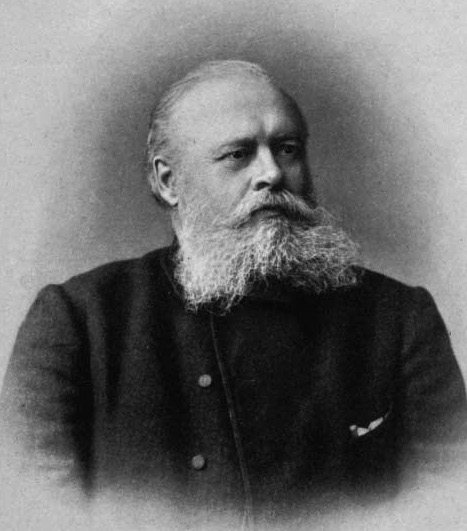
\includegraphics[width=\linewidth]{images/book2/markovnikov.jpg}
\end{minipage}\hfill
\begin{minipage}[t]{0.76\linewidth}\vspace{0pt}
Vladimir Markovnikov formuleerde zijn regel in de negentiende eeuw, op
basis van de producten die hij en anderen waarnamen, lang voordat
\omterm{def:b1:electronic-effects:intermediates}{carbokationen} of \omterm{def:b1:electronic-effects:curly-arrow}{gebogen pijlen} bestonden: een regelmaat van de natuur,
opgeschreven voordat ze verklaard kon worden. De moderne formulering via
de stabiliteit van \omterm{def:b1:electronic-effects:intermediates}{carbokationen} toont wat een mechanisme aan een
empirische regel toevoegt: het zegt wanneer de regel zou moeten falen.
(Portret uit een in memoriam gepubliceerd in 1905, publiek domein,
Wikimedia Commons.)
\end{minipage}
\end{history}

\section{Oefeningen}

\begin{exercise}[$\star$]\label{exo:b1:electrophilic-additions:1}
Geef het hoofdproduct van: propeen + HCl; 2-methylpropeen + HBr;
1-methylcyclohexeen + HBr; but-2-yn + één equivalent HCl.
\end{exercise}

\begin{exercise}[$\star$]\label{exo:b1:electrophilic-additions:2}
Schrijf de producten op van broom met etheen, cyclohexeen en propeen.
Geef hun naam.
\end{exercise}

\begin{exercise}[$\star$]\label{exo:b1:electrophilic-additions:3}
Welke alcohol geeft de zuurgekatalyseerde \omterm{def:b1:electrophilic-additions:hydration}{hydratatie} van elk alkeen:
propeen, 2-methylpropeen, methyleencyclohexaan?
\end{exercise}

\begin{exercise}[$\star$]\label{exo:b1:electrophilic-additions:4}
Welke van deze verbindingen reageren met natriumamide: propyn, but-2-yn,
propeen, ethanol? Schrijf de reacties op.
\end{exercise}

\begin{exercise}[$\star\star$]\label{exo:b1:electrophilic-additions:5}
Schrijf het volledige mechanisme op van de \omterm{def:b1:electrophilic-additions:hydration}{hydratatie} van
2-methylpropeen met \omterm{def:b1:electronic-effects:curly-arrow}{gebogen pijlen}, en verklaar waarom de omgekeerde
reactie in heet geconcentreerd zuur begunstigd is.
\end{exercise}

\begin{exercise}[$\star\star$]\label{exo:b1:electrophilic-additions:6}
Verklaar met het postulaat van Hammond waarom 2-methylpropeen veel
sneller met HCl reageert dan propeen.
\end{exercise}

\begin{exercise}[$\star\star$]\label{exo:b1:electrophilic-additions:7}
Broom reageert met cyclohexeen. Toon aan dat het product
\textit{trans}-1,2-dibroomcyclohexaan is, en zeg of het \omterm{def:b1:stereochemistry-in-depth:stereocentre}{chiraal} is en of
het product optisch actief is.
\end{exercise}

\begin{exercise}[$\star\star$]\label{exo:b1:electrophilic-additions:8}
Stel een mechanisme voor van de additie van HCl aan 3-methylbut-1-een die
vooral 2-chloor-2-methylbutaan geeft.
\end{exercise}

\begin{exercise}[$\star\star$]\label{exo:b1:electrophilic-additions:9}
Stel een synthese voor van hex-2-yn uit propyn en een halogeenalkaan, en
van 1-fenylbut-2-yn-1-ol uit propyn en benzaldehyde.
\end{exercise}

\begin{exercise}[$\star\star\star$]\label{exo:b1:electrophilic-additions:10}
Bewijs met tekeningen de stereochemie van de broomadditie aan de twee
but-2-enen: bromoniumion, anti-aanval op elk koolstofatoom, \omterm{def:b1:stereochemistry-in-depth:representations}{weergave
volgens Cram} van de producten, descriptoren. Tel de \omterm{def:b1:stereochemistry-in-depth:isomers}{stereo-isomeren} die
in elk geval ontstaan.
\end{exercise}

\begin{exercise}[$\star\star\star$]\label{exo:b1:electrophilic-additions:11}
Broomwater geeft met propeen 1-broompropaan-2-ol als hoofdproduct.
Verklaar de regiochemie: waarom valt water het meest gesubstitueerde
koolstofatoom van het bromoniumion aan?
\end{exercise}

\begin{exercise}[$\star\star\star$]\label{exo:b1:electrophilic-additions:12}
Een koolwaterstof \ce{C5H10} ontkleurt broomwater en addeert HBr tot
2-broom-2-methylbutaan; zijn \omterm{def:b1:electrophilic-additions:hydration}{hydratatie} geeft 2-methylbutaan-2-ol. Vind
twee mogelijke structuren en stel een manier voor om ze te onderscheiden.
\end{exercise}

\section{Probleem: twee butenen en broom}

\begin{problem}[{Weekendprobleem --- de twee but-2-enen, het
bromoniummechanisme, meso- en racemische dibromiden, hun optische
rotatie en de verkregen massa}]
\label{pb:b1:electrophilic-additions:1}
Een laboratorium heeft twee flessen but-2-een, één zuiver \cip{Z}, één
zuiver \cip{E}, en behandelt \qty{5.60}{g} van elk met broom in
dichloormethaan. Molaire massa's (\unit{g/mol}): \ce{C4H8} 56.0,
\ce{Br2} 159.8, \ce{C4H8Br2} 215.8.

\medskip
\noindent\textbf{Deel I --- De twee alkenen.}
\begin{enumerate}
  \item Teken \cip{Z}- en \cip{E}-but-2-een en verantwoord de
        descriptoren.
  \item Zijn het \omterm{def:b1:stereochemistry-in-depth:isomers}{stereo-isomeren}? \omterm{def:b1:stereochemistry-in-depth:enantiomers}{Enantiomeren} of \omterm{def:b1:stereochemistry-in-depth:enantiomers}{diastereomeren}?
  \item Waarom gaan ze bij kamertemperatuur niet in elkaar over?
  \item Welke is het stabielst, en waarom?
  \item Schrijf de totale vergelijking op van de additie van broom.
  \item Hoeveel stereocentra heeft 2,3-dibroombutaan? Hoeveel
        \omterm{def:b1:stereochemistry-in-depth:isomers}{stereo-isomeren} hoogstens, en hoeveel in werkelijkheid?
\end{enumerate}

\medskip
\noindent\textbf{Deel II --- Het mechanisme.}
\begin{enumerate}[resume]
  \item Schrijf de vorming van het bromoniumion op met \omterm{def:b1:electronic-effects:curly-arrow}{gebogen pijlen}.
  \item Waarom ontstaat er een overbrugd bromoniumion in plaats van een
        open \omterm{def:b1:electronic-effects:intermediates}{carbokation}?
  \item Schrijf de opening van het ion door bromide op.
  \item Waarom valt bromide aan vanaf de kant tegenover de brug?
  \item Wat voor additie is het resultaat?
  \item Waarom is het oplosmiddel dichloormethaan en geen water?
\end{enumerate}

\medskip
\noindent\textbf{Deel III --- De producten.}
\begin{enumerate}[resume]
  \item Uit \cip{E}-but-2-een: teken het product van de aanval op C2 en
        geef de descriptoren van C2 en C3.
  \item Hetzelfde voor de aanval op C3. Vergelijk.
  \item Toon aan dat het product meso is.
  \item Uit \cip{Z}-but-2-een: teken de twee producten en hun
        descriptoren.
  \item In welke verhoudingen ontstaan ze? Geef het mengsel een naam.
  \item Is de reactie stereospecifiek? Verantwoord.
\end{enumerate}

\medskip
\noindent\textbf{Deel IV --- Rotatie en massa.}
\begin{enumerate}[resume]
  \item Welke optische rotatie vertoont het product van het
        \cip{Z}-alkeen?
  \item Bereken de hoeveelheid stof van elk alkeen.
  \item Bereken de massa dibromide die uit elk ervan verwacht wordt bij
        een \omterm{def:b1:extent-q-and-k:fractional-extent}{rendement} van \qty{85}{\percent}.
  \item Geef de \omterm{def:b1:stereochemistry-in-depth:optical-activity}{specifieke rotatie} van het dibromide verkregen uit
        \cip{E}-but-2-een, en de verkregen massa ervan.
\end{enumerate}
\end{problem}
